\documentclass[tikz,border=10pt]{standalone}
\usepackage{tikz}
\usetikzlibrary{arrows.meta,calc}

\definecolor{figazul}{RGB}{2,132,199}
\definecolor{figrojo}{RGB}{220,38,38}
\definecolor{figverde}{RGB}{22,163,74}

\begin{document}
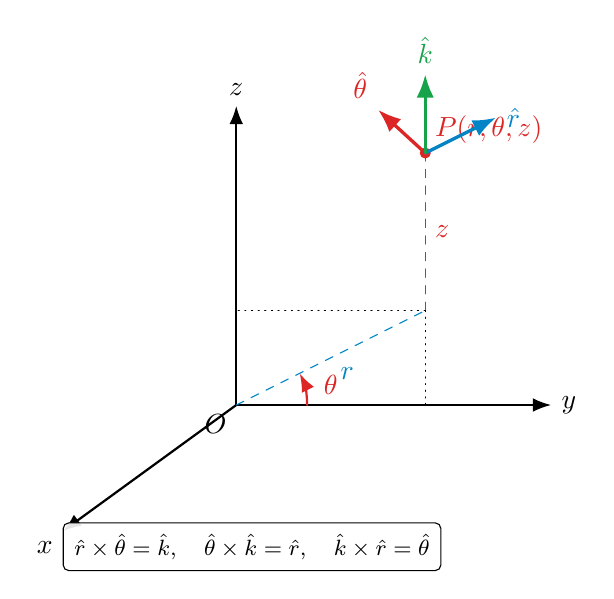
\begin{tikzpicture}[>=Latex, line cap=round, line join=round]
  % Ejes cartesianos
  \draw[->, thick] (0,0) -- (4,0) node[right] {$y$};
  \draw[->, thick] (0,0) -- (0,3.8) node[above] {$z$};
  \draw[->, thick] (0,0) -- (-2.2,-1.6) node[below left] {$x$};
  \node[below left] at (0,0) {$O$};

  % Coordenadas del punto P en perspectiva
  % Plano xy: r a ángulo phi
  \coordinate (O) at (0,0);
  \coordinate (Pxy) at (2.4, 1.2);
  \coordinate (P) at (2.4, 3.2);

  % Proyección en plano xy
  \draw[dashed, thin, color=figazul] (O) -- (Pxy) node[midway, below right, color=figazul] {$r$};
  \draw[dashed, thin, color=figrojo] (Pxy) -- (P) node[midway, right, color=figrojo] {$z$};
  \draw[dotted, thin] (Pxy) -- (2.4, 0);
  \draw[dotted, thin] (Pxy) -- (0, 1.2);

  % Arco para ángulo theta
  \draw[->, thick, color=figrojo] (0.9,0) arc (0:26.5:0.9);
  \node[color=figrojo] at (1.2, 0.25) {$\theta$};

  % Punto P(r, theta, z)
  \fill[color=figrojo] (P) circle (2pt);
  \node[above right, color=figrojo] at (P) {$P(r, \theta, z)$};

  % Versores canónicos en P
  % r_hat: a lo largo de OPxy
  \draw[->, very thick, color=figazul] (P) -- ($(P) + (0.9, 0.45)$) node[right, color=figazul] {$\hat{r}$};
  % theta_hat: perpendicular a r_hat en plano horizontal (-0.45, 0.9)
  \draw[->, very thick, color=figrojo] (P) -- ($(P) + (-0.6, 0.55)$) node[above left, color=figrojo] {$\hat{\theta}$};
  % k_hat: vertical
  \draw[->, very thick, color=figverde] (P) -- ($(P) + (0, 1.0)$) node[above, color=figverde] {$\hat{k}$};

  % Relación de versores
  \node[draw, rounded corners=2pt, inner sep=4pt, fill=white, fill opacity=0.9, text opacity=1, font=\footnotesize] at (0.2, -1.8) 
    {$\hat{r} \times \hat{\theta} = \hat{k}, \quad \hat{\theta} \times \hat{k} = \hat{r}, \quad \hat{k} \times \hat{r} = \hat{\theta}$};
\end{tikzpicture}
\end{document}
